\documentclass{report}

\usepackage{amsmath}
\usepackage{graphicx} % to insert images
\graphicspath{{../pdf/}{/Users/rutviksayankar/Repos/ECE445_SP24/TACheckIn/Rutvik/IndividualProgressReport/Images}} % setting up path for image storage
\usepackage{hyperref} % allows table of contents to be clickable to sections
\hypersetup{
    colorlinks,
    citecolor=blue,
    filecolor=blue,
    linkcolor=blue,
    urlcolor=blue
}

\title{ECE 445: Senior Design Lab \\ Final Report \\ Oxygen Delivery Robot} % Sets article title

\author {
    \textbf{Team 27} \\ 
    \textit{Sayankar, Rutvik}\\
    \textit{rutviks2@illinois.edu} \\
    \hfill \\ 
    \textit{Dunican, Aidan}\\
    \textit{dunican2@illinois.edu} \\
    \hfill \\ 
    \textit{Kalyniouk, Nazar}\\
    \textit{nazark2@illinois.edu} \\
    \hfill \\ 
    \textbf{Under the guidance of} \\ 
    \textit{Subramaniam, Selva} \\
    \textit{ss170@illinois.edu} 
} 
\date{\today} % Sets date for date compiled

% The preamble ends with the command \begin{document}
\begin{document}
    \maketitle % creates title using information in preamble (title, author, date)
    
    \pagebreak
    \tableofcontents % creates table of contents
    \pagebreak

    \section{Terms and Keywords}
    \vspace{0.8cm}
    \begin{itemize}
        \item ChILD - Children's Interstitial and Diffuse Lung Disease
        \item PCB – Printed Circuit Board
        \item OWB - Three-Wheeled Omni-Wheel Bot
        \item UWB - Ultra-wideband is a radio technology that can use a very low energy level for short-range, high-bandwidth communications over a large portion of the radio spectrum.
        \item ESP32 - A series of low-cost, low-power system-on-a-chip microcontrollers with integrated Wi-Fi and dual-mode Bluetooth.
        \item RPM - Revolutions per minute
        \item GPIO - General-purpose input/output
        \item SPI - Serial Peripheral Interface
        \item PWM - Pulse-width modulation
        \item MPH - Miles per hour
        \item OpenCV - (Open Source Computer Vision Library) is an open source computer vision and machine learning software library.
        \item OpenPose - Real-time multi-person keypoint detection library for body, face, hands, and foot estimation.
        \item TDoA - Time Difference of Arrival 
        \item ToF - Time of Flight
    \end{itemize}

    \pagebreak

    \chapter{Introduction}
    \section{Team Project Overview}
    Children's interstitial and diffuse lung disease (ChILD) is a collection of diseases or disorders. These diseases cause a thickening of the interstitium (the tissue that extends throughout the lungs) due to scarring, inflammation, or fluid buildup \cite{ChILD-2022}. This eventually affects a patient’s ability to breathe and distribute enough oxygen to the blood. Numerous children experience the impact of this situation, requiring supplemental oxygen for their daily activities. It hampers the mobility and freedom of young infants, diminishing their growth and confidence. Moreover, parents face an increased burden, not only caring for their child but also having to be directly involved in managing the oxygen tank as their child moves around.

    Given the absence of relevant solutions in the current market, our project aims to ease the challenges faced by parents and provide the freedom for young children to explore their surroundings. As a proof of concept for an affordable solution, we propose a three-wheeled omnidirectional mobile robot capable of supporting a filled M-6 oxygen tank. We plan to implement two localization subsystems to ensure redundancy and enhance child safety. The first subsystem utilizes ultra-wide band (UWB) transceivers for triangulating the child's location relative to the robot in indoor environments, this is similar to how Apple AirTags triangulate their location relative to an iPhone \cite{airtag_uwb} (although AirTags use a combination of UWB and Bluetooth triangulation \cite{airtag_ble}). The second subsystem makes use of a desktop web camera which streams video to a Raspberry Pi where it will leverage open-source object tracking libraries to improve our directional accuracy in tracking a child. The final main subsystem focuses on the drive train, chassis and close range object detection of the robot.

    \chapter{Individual Design Work}
    \section{Design Considerations \& Diagrams}

    \subsection{PCB Design}
    The design of the schematic of the PCB was done due to the main required components and what all was needed to ensure the components were properly powered and able to communicate, I completed all of the parts except for the power regulation circuits. The layout of the PCB required a different style of thought (\ref{fig:MainBoardv1.1_Layout}). I had to consider how the board would be used, what connections would come out of the board and in what direction they would need to face. This is important as it would help prevent wiring from getting messy and therefore preventing any possible issues that may arrise from having messy wiring. I chose to keep the motor power, PWM and encoder wiring close together on the layout. Each of those things are also facing the same direction, this should help ensure that wiring won't get tangled together. The connections for the SPI bus are all also facing the same direction. Finally, the power input from the battery is far away from other connections, and should not get mixed up with anything else on the board.

    Knowing the importance of visual indicators during debugging, I have added LEDs for each power level to help indicate when the circuit is live and when power has been properly stepped down. Aside from general PCB organization, a very helpful item that has been added is the QR code linking to our project Github that is on the board. This gives us the ability to quickly check for something incase any issue arrises and it gives a third party observer a place to learn more about the project.

    Finally, understanding the importance of knowing the connections during debugging I've ensured that I have labeled as much as possible in terms of connectors and pins. There should be no confusion when wiring or PCB assembly in terms of what goes where.

    \begin{figure}[ht!]
        \centering
        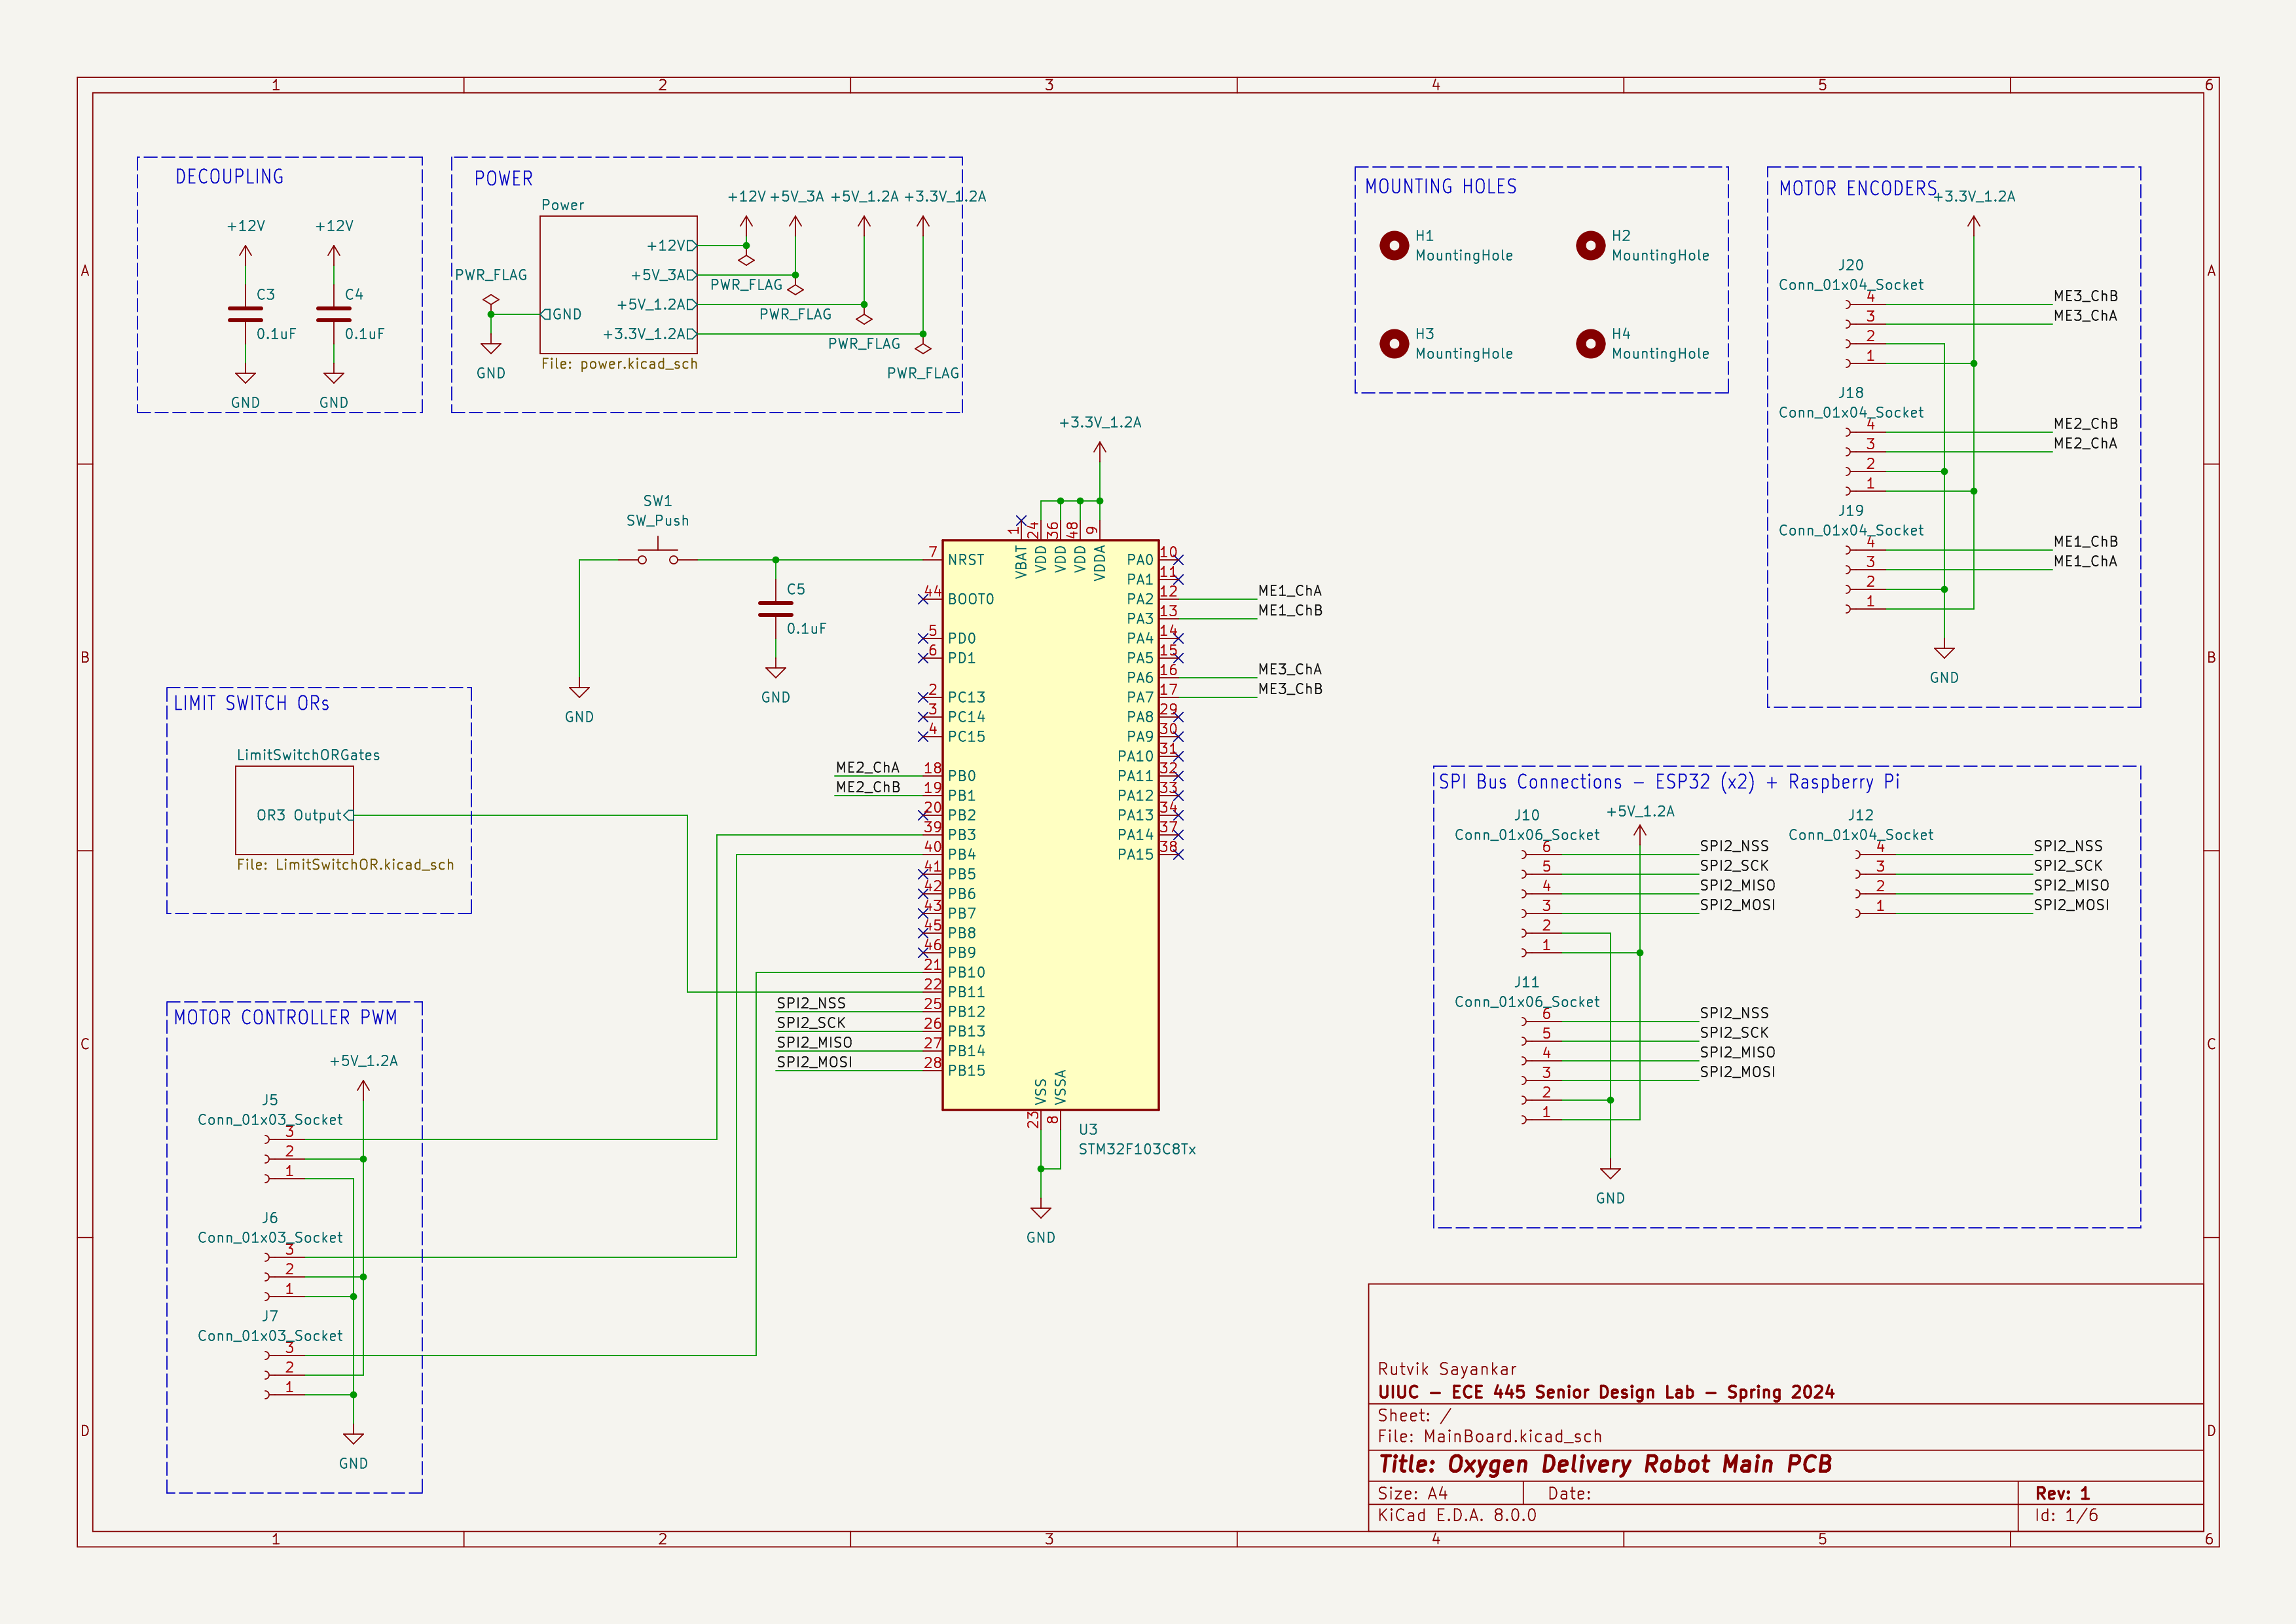
\includegraphics[width=0.6\textwidth]{MainSchematic.png}
        \caption{MainBoardv1.1 Main Schematic}
        \label{fig:MainSchematic}
    \end{figure}

    \begin{figure}[ht!]
        \centering
        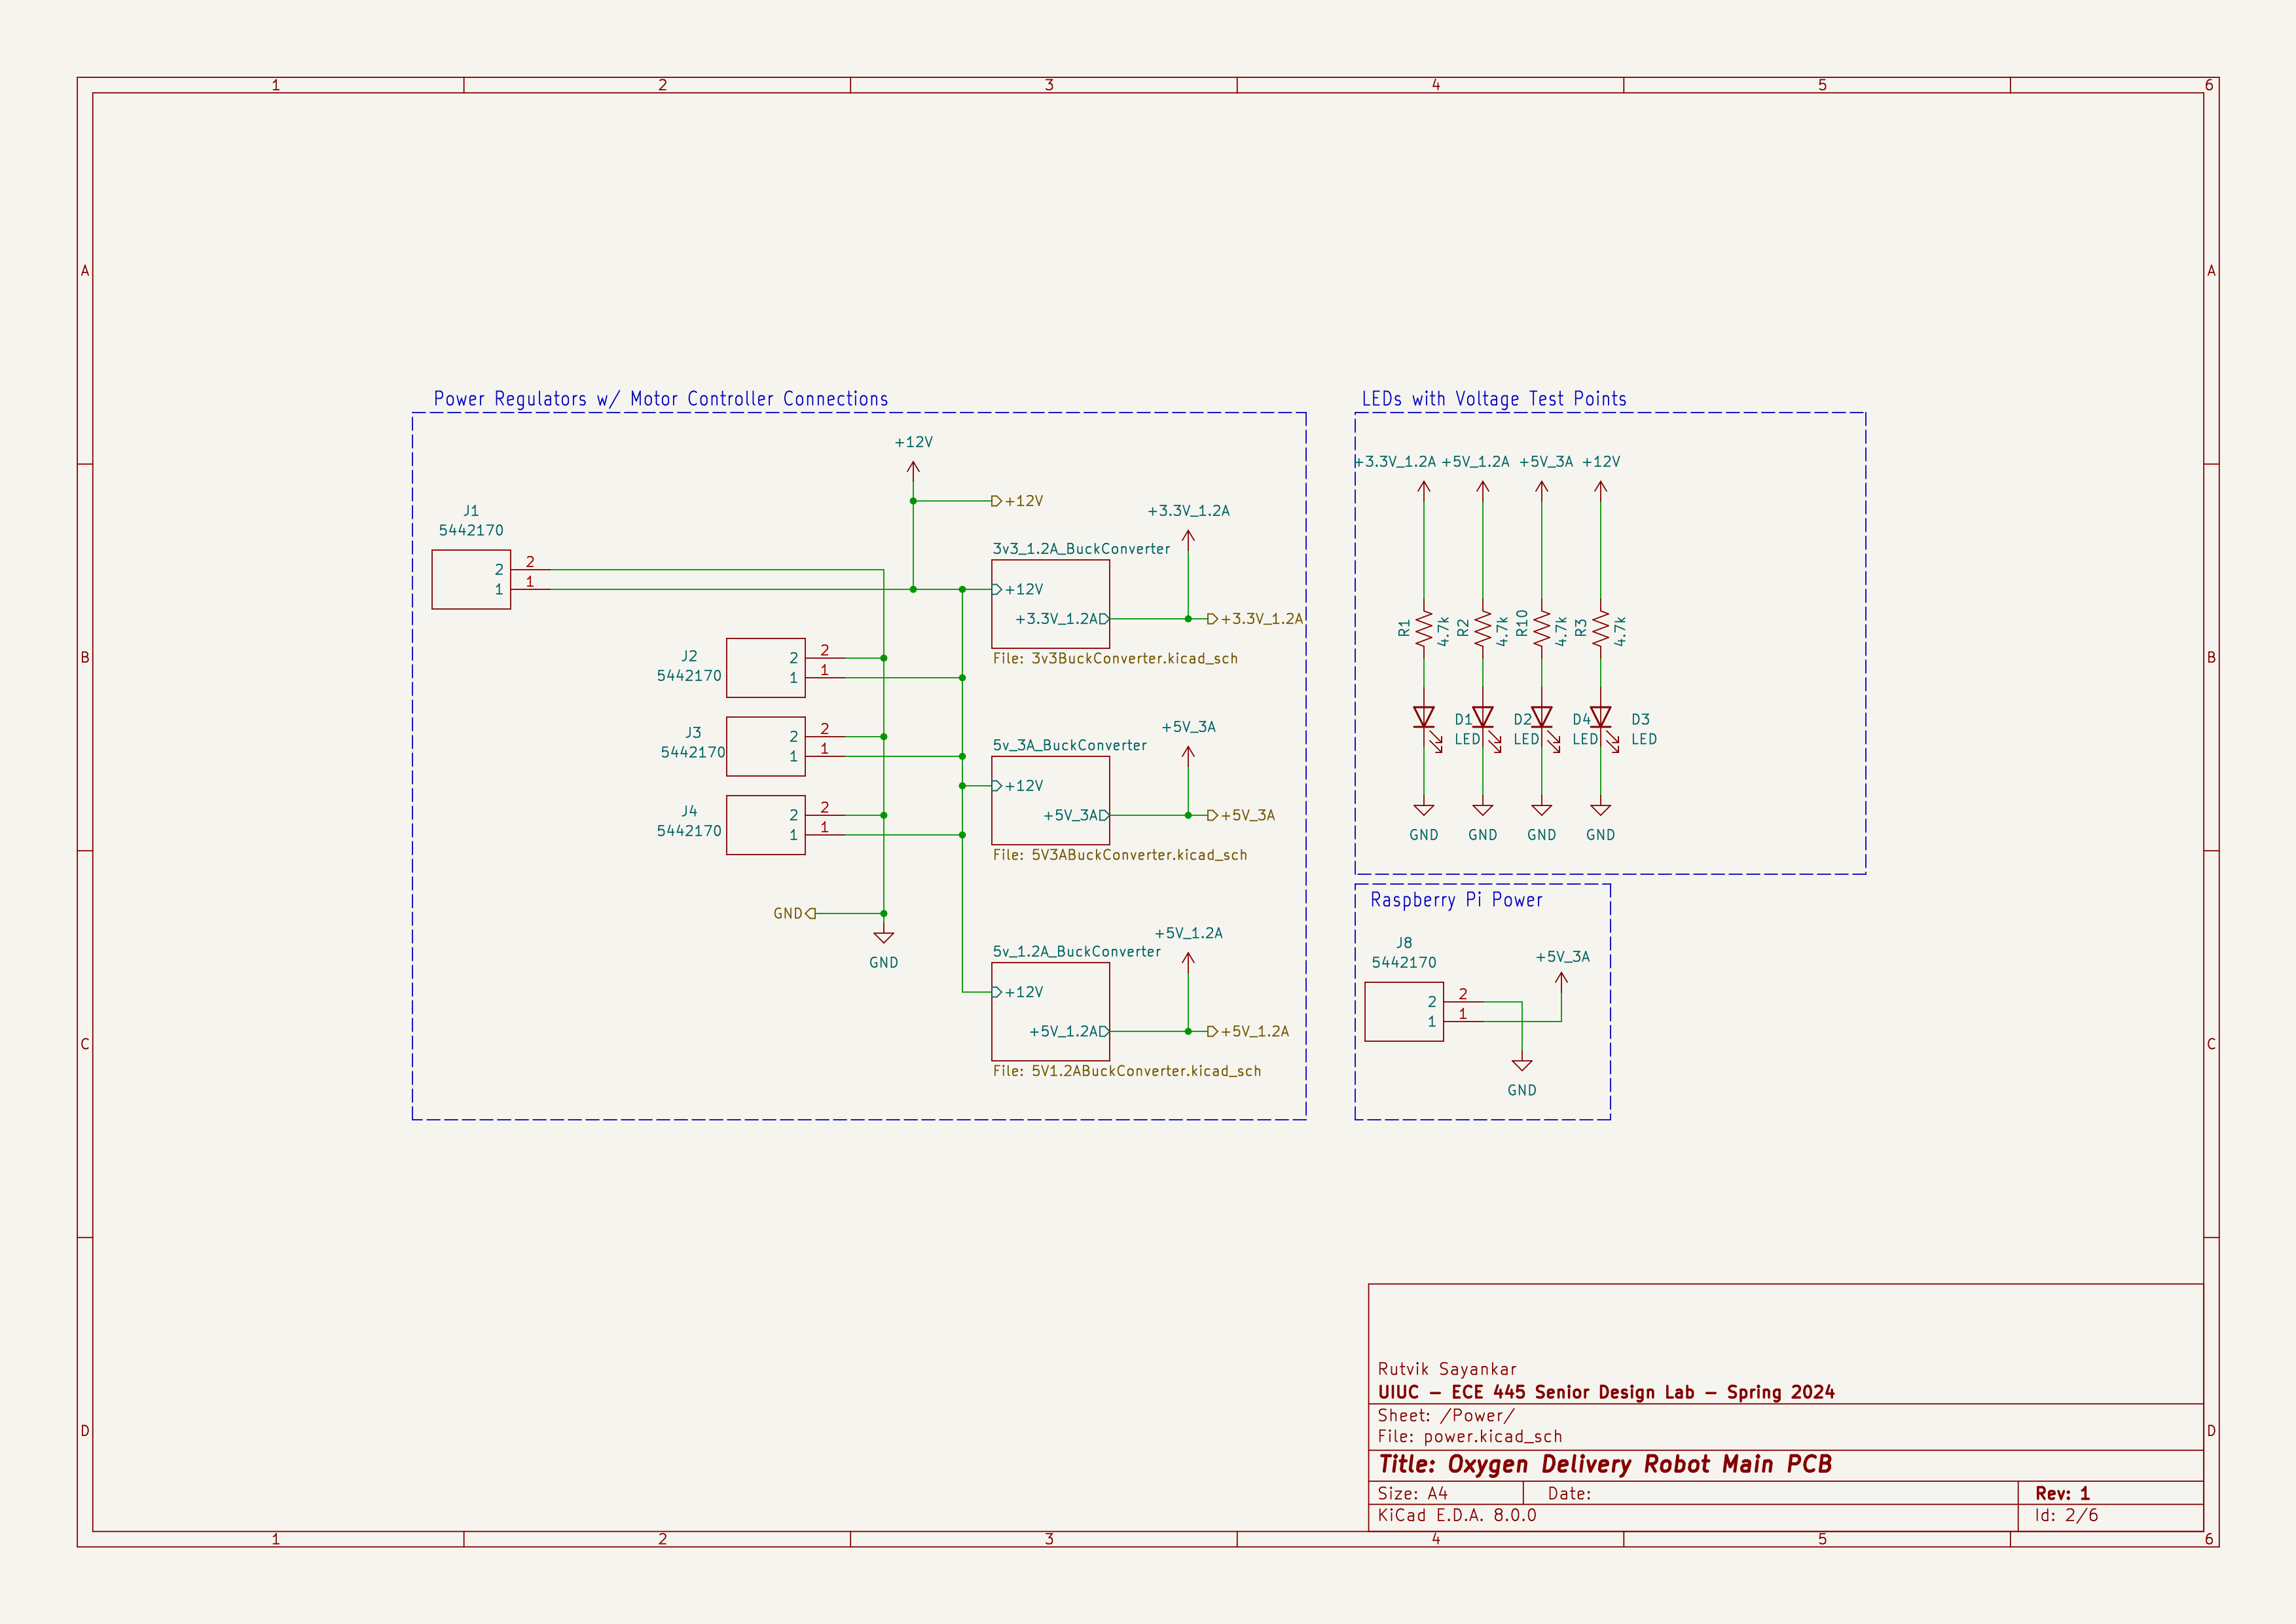
\includegraphics[width=0.6\textwidth]{PowerSchematic.png}
        \caption{MainBoardv1.1 Power Schematic}
        \label{fig:PowerSchematic}
    \end{figure}

    \begin{figure}[ht!]
        \centering
        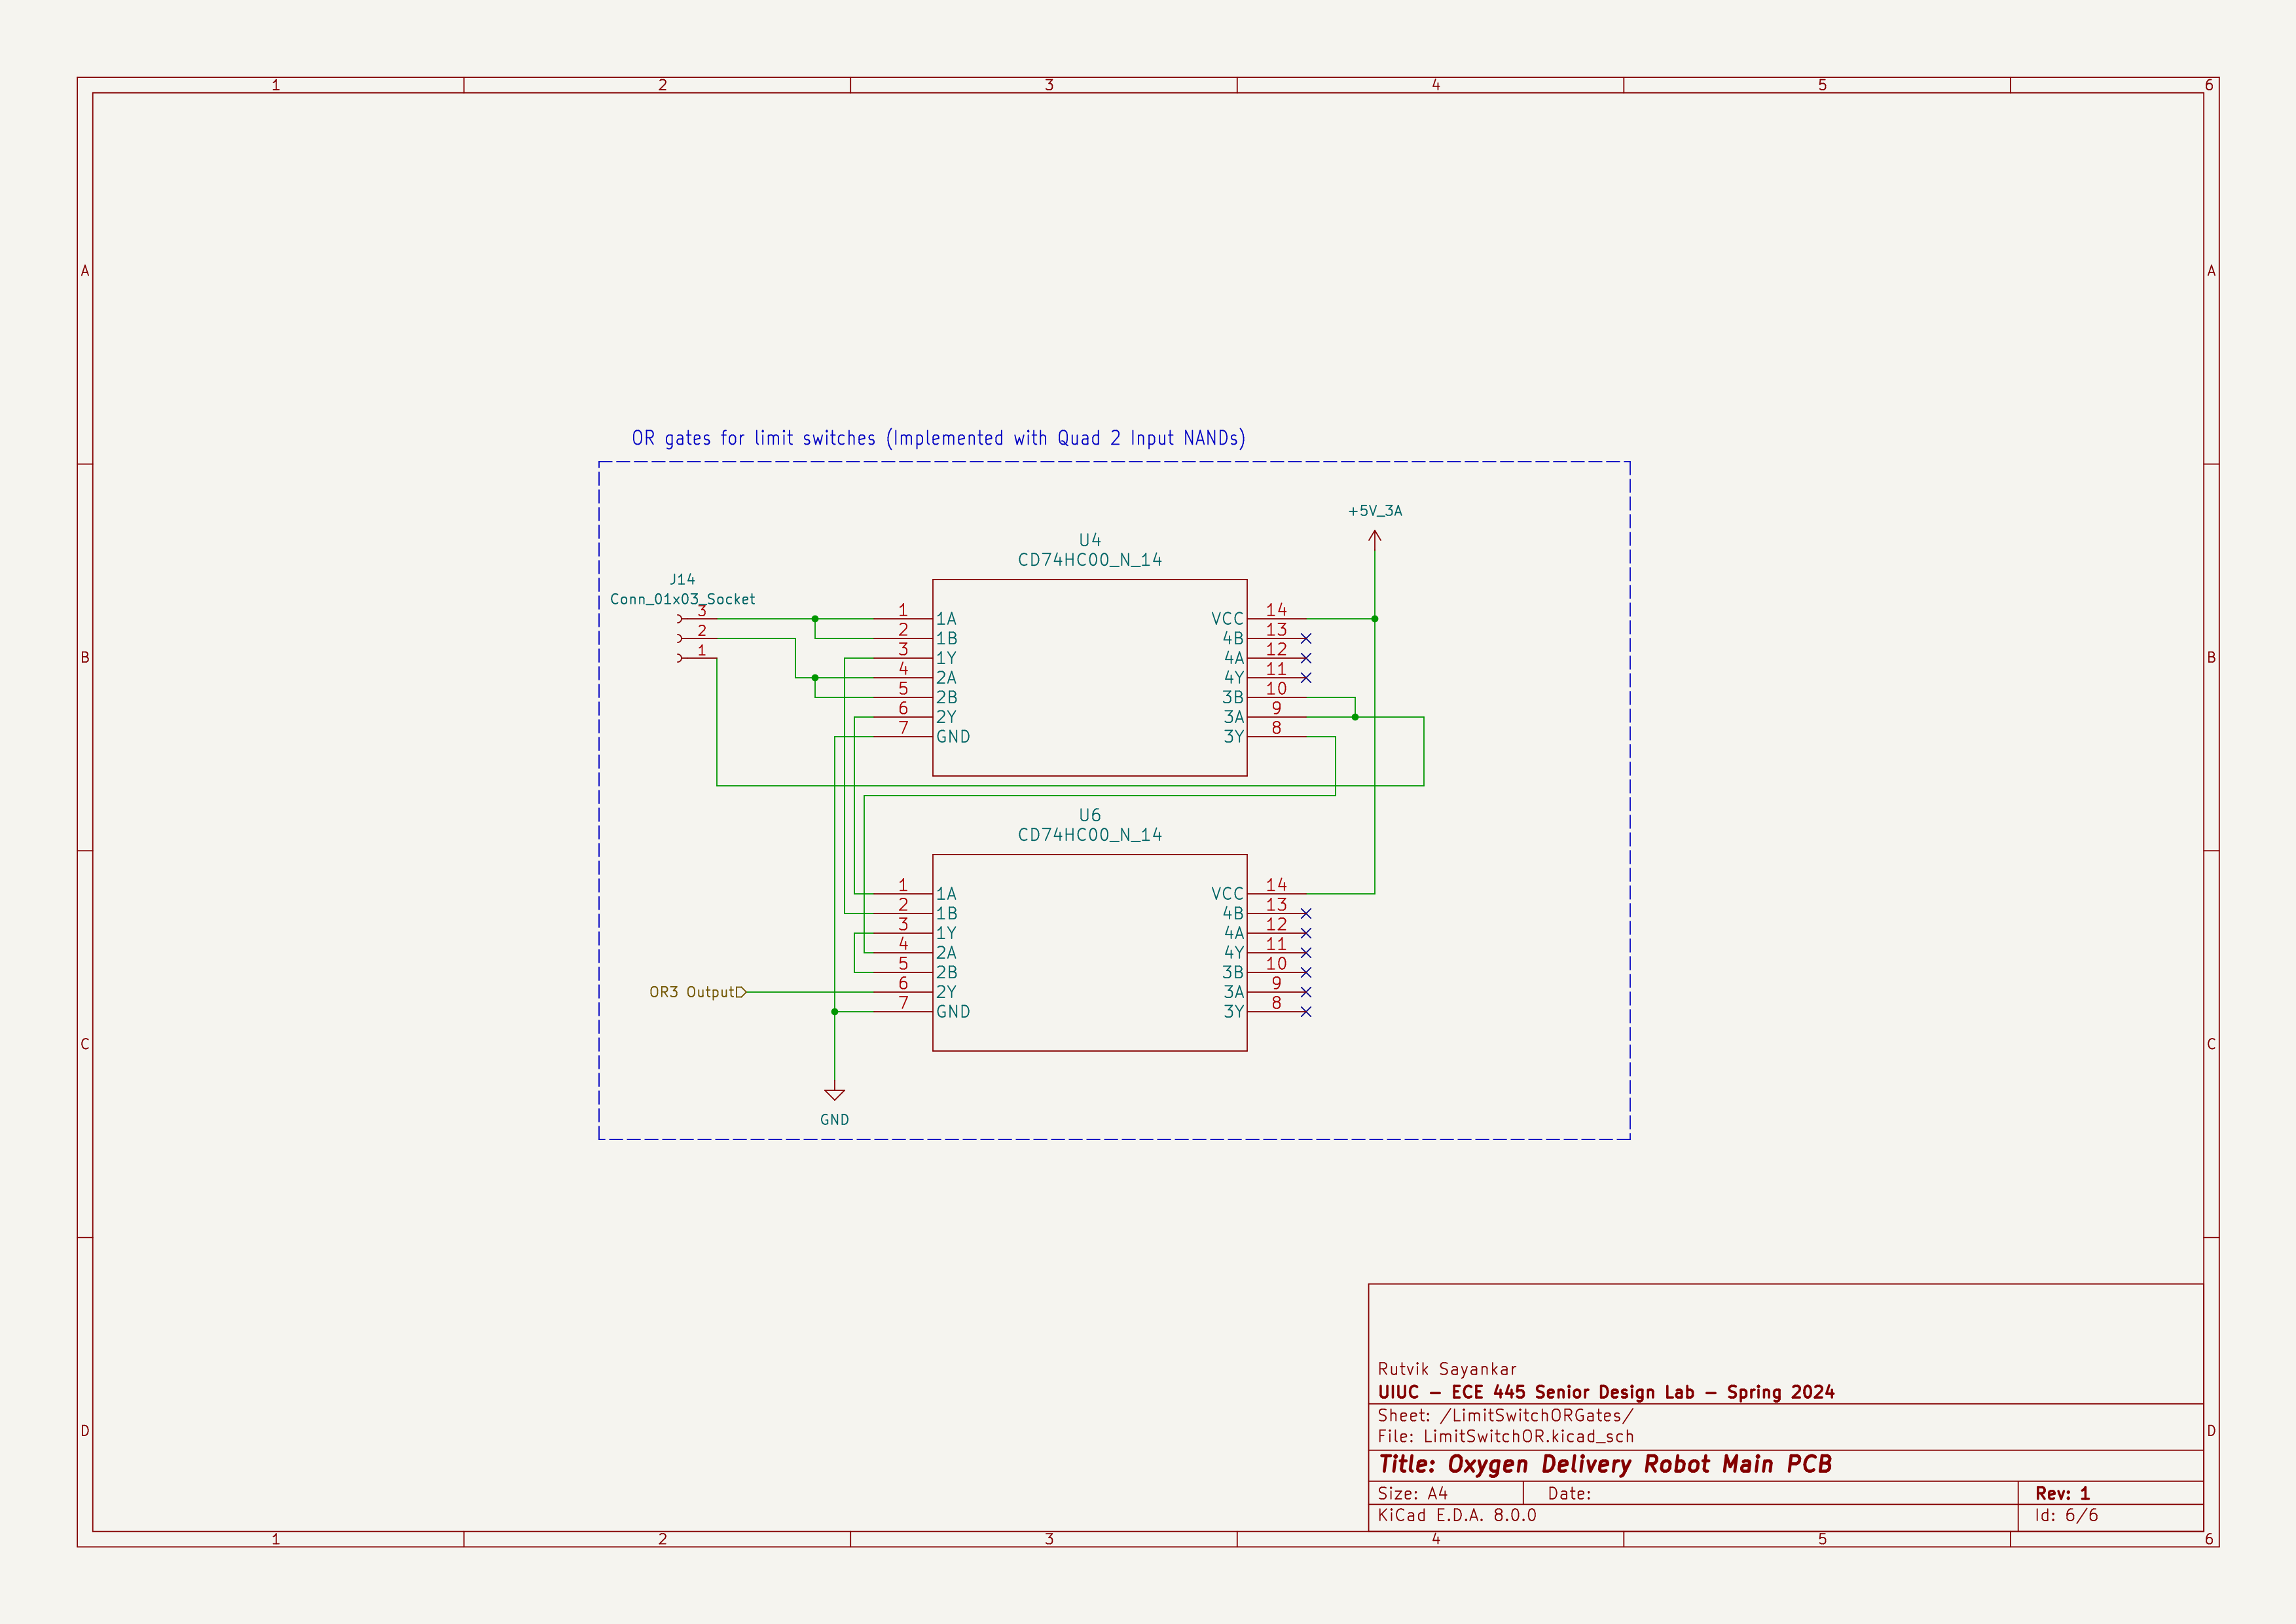
\includegraphics[width=0.6\textwidth]{ORSchematic.png}
        \caption{MainBoardv1.1 OR3 Gate Schematic}
        \label{fig:ORSchematic}
    \end{figure}

    \begin{figure}[ht!]
        \centering
        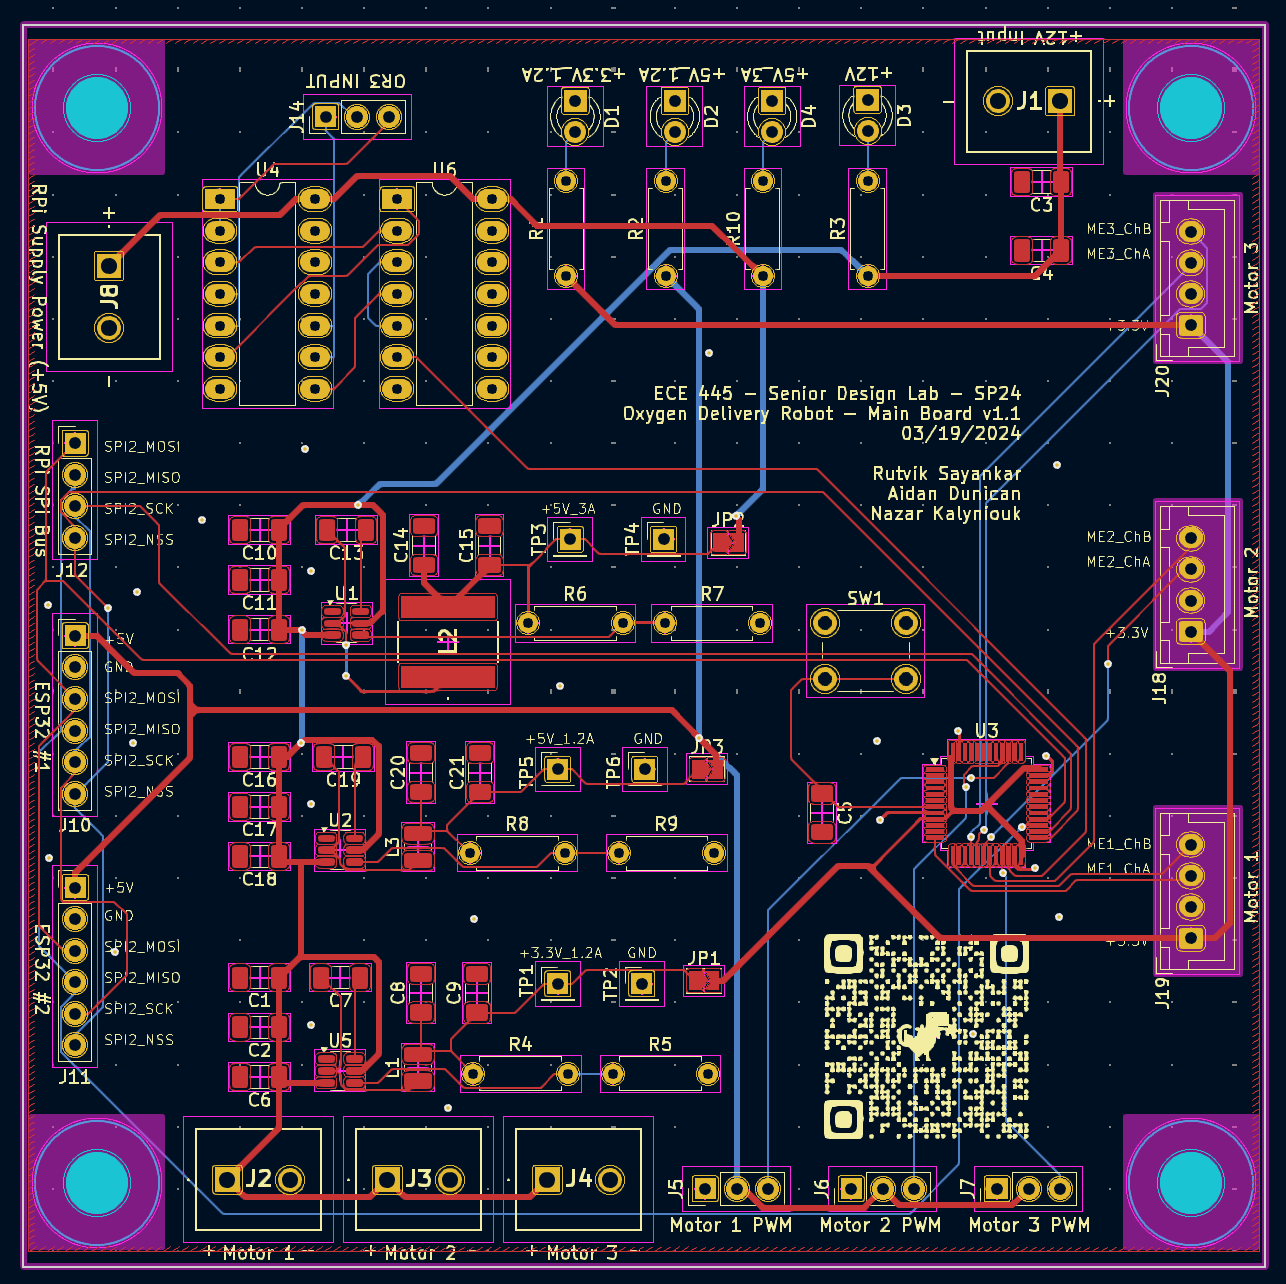
\includegraphics[width=0.8\textwidth]{KiCAD_MainBoardv2_Screenshot.png}
        \caption{MainBoardv1.1 Board Layout}
        \label{fig:MainBoardv1.1_Layout}
    \end{figure}
    
    \subsection{UWB System}
    After ordering the UWB transceivers from \href{https://www.makerfabs.com/esp32-uwb-dw3000.html}{MakerFabs} I was able to get started on testing out the accuracy of the transceivers, and seeing how I would be able to send packets back and forth. I began by implementing a simple ranging test (\ref{fig:UWBRanging}). With some moving around of the transceivers I was able to get a fairly accurate reading of the distance between two transceivers (\ref{fig:UWBRangingSerialMonitor}).

    I am currently in progress tweaking the triangulation code with three transceivers, to get a location relative to two anchors.

    \begin{figure}[ht!]
        \centering
        \includegraphics[width=0.8\textwidth]{UWB_30cm.png}
        \caption{UWB Ranging Test}
        \label{fig:UWBRanging}
    \end{figure}

    \begin{figure}[ht!]
        \centering
        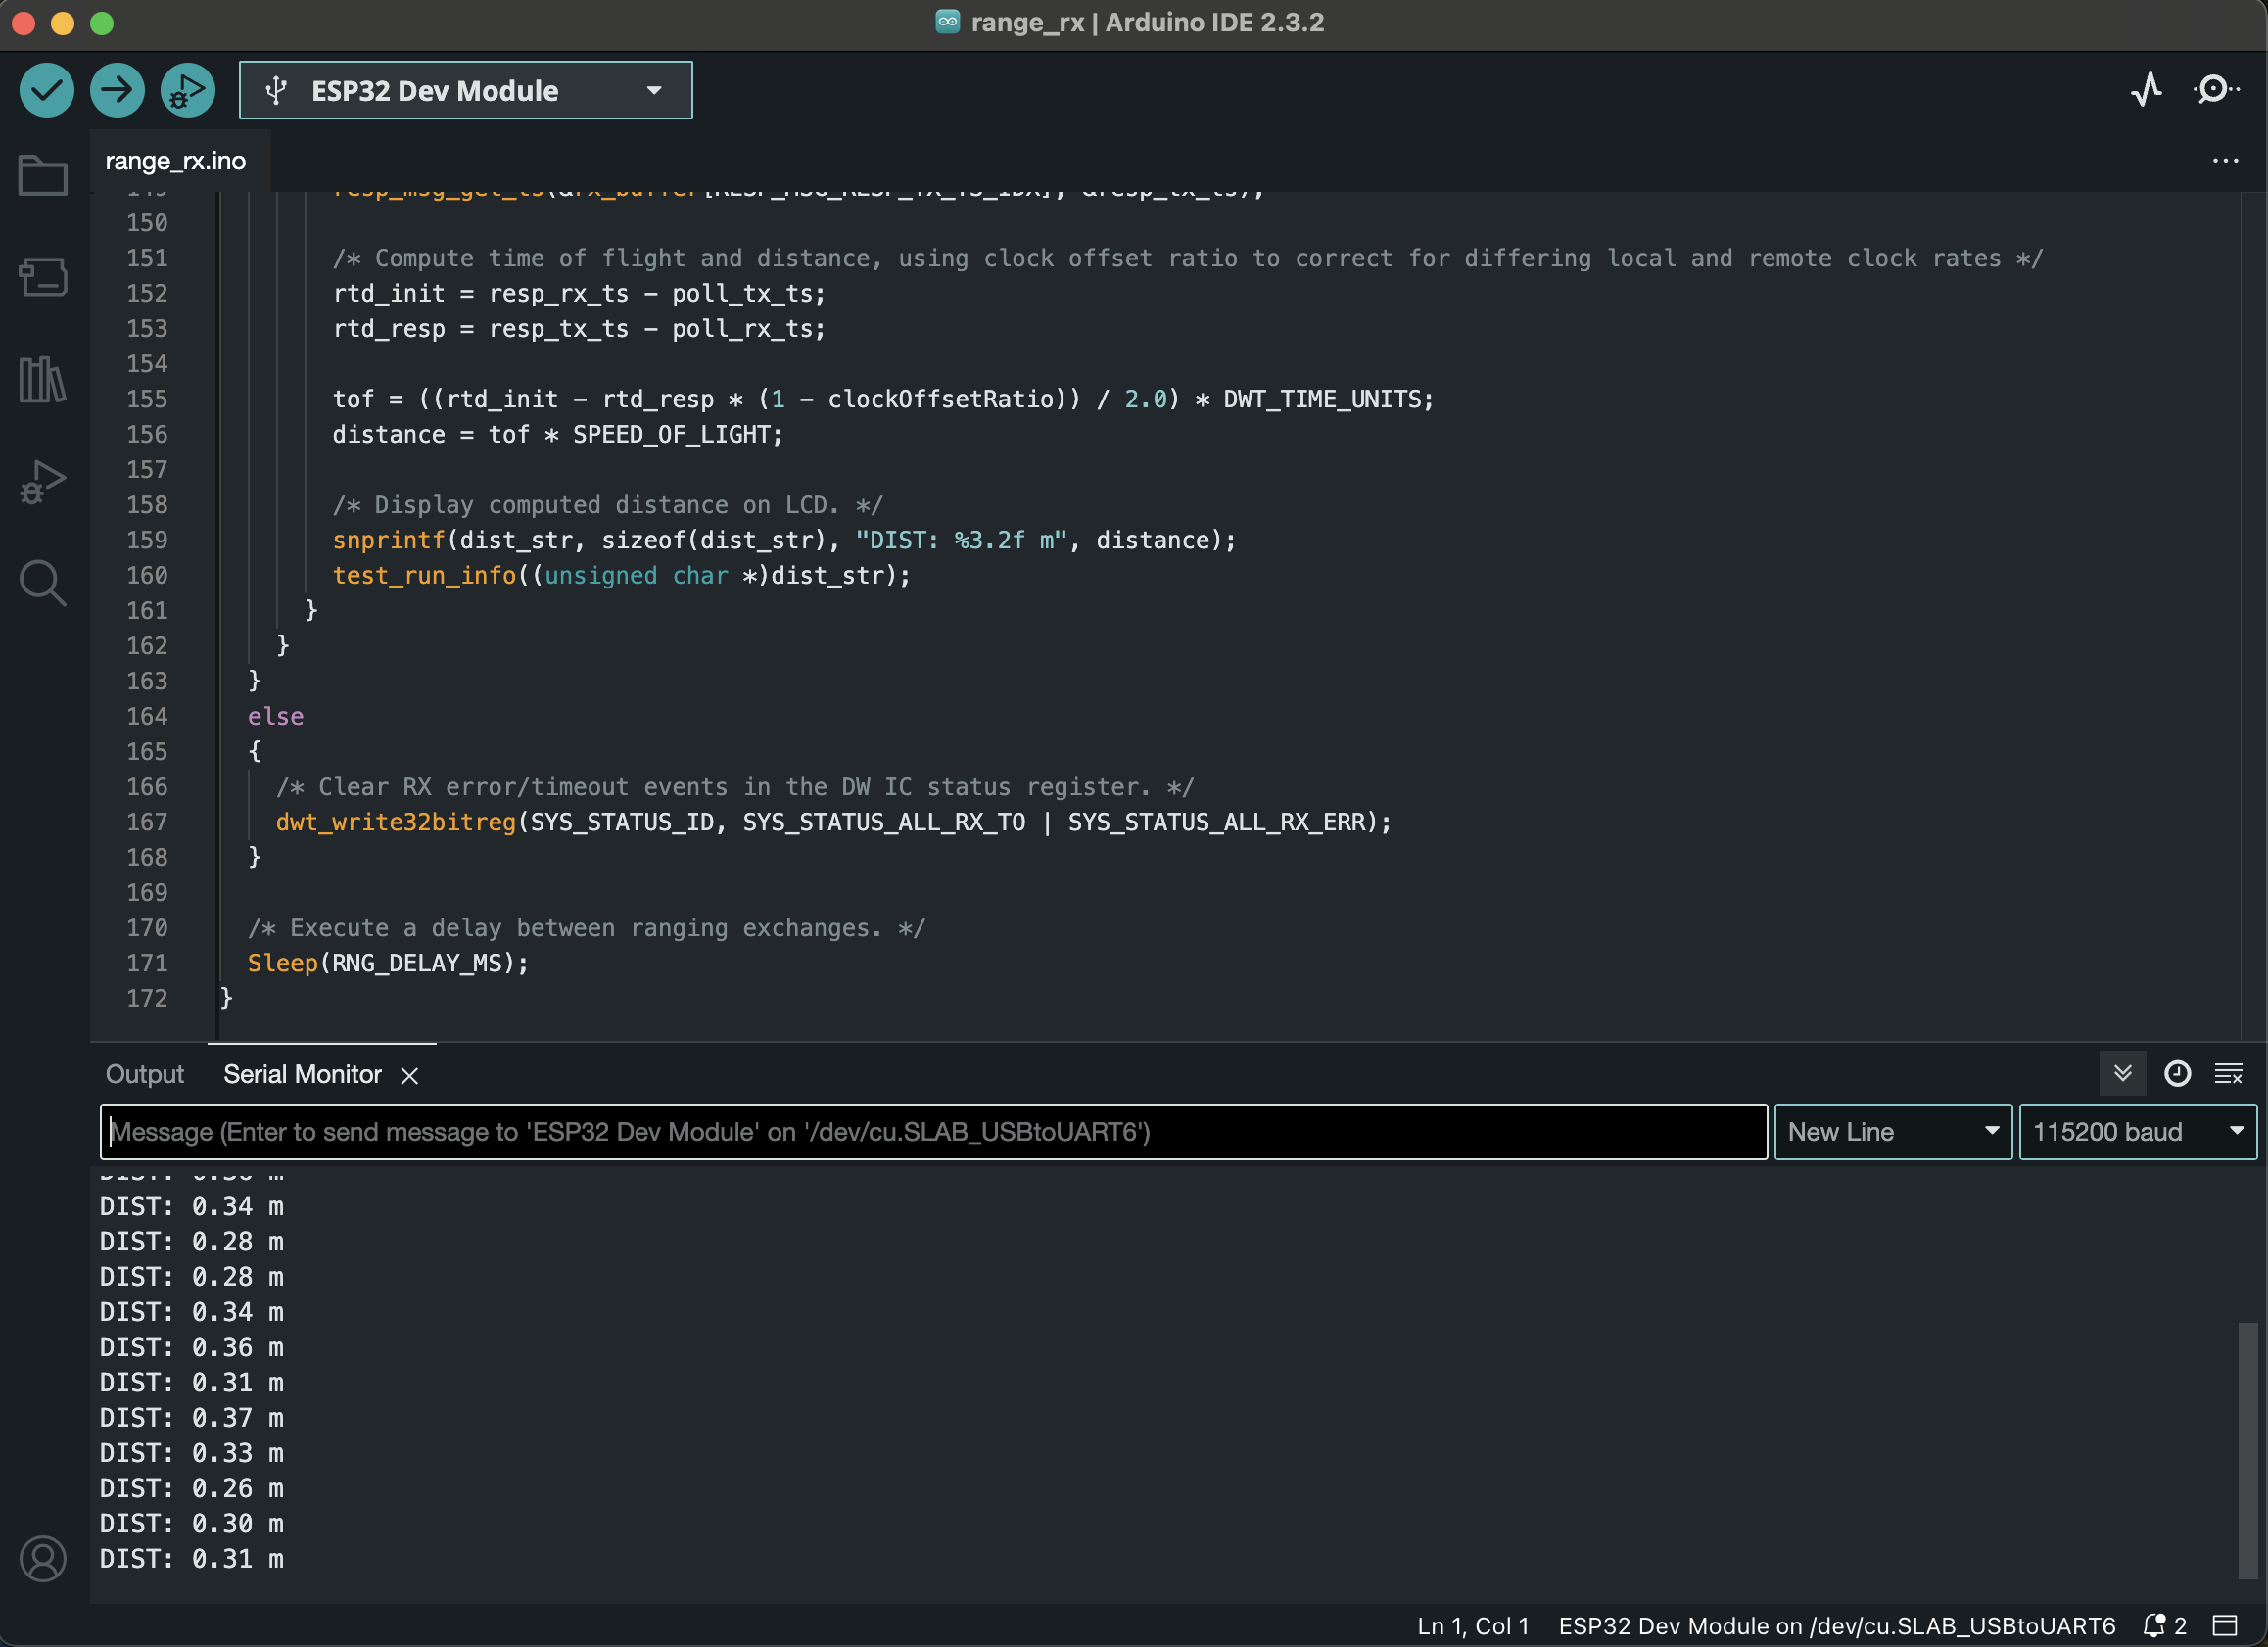
\includegraphics[width=0.8\textwidth]{UWB_30cm_SerialMonitor.png}
        \caption{UWB Ranging Test - Serial Monitor Output}
        \label{fig:UWBRangingSerialMonitor}
    \end{figure}

    \subsection{Bumper Limit Switch \& 3D Printing}

    I have worked with Aidan on desiging the bumper limit switch. Mainly I have been focused on the 3D printablity of the part. Testing the prints, and seeing what tweaks need to be made. Currently we're focusing on modularity of the bumper. Creating a screw connector between the actual bumper and the limit switch (\ref{fig:LimitSwitchScrewTerminal}). This way if something gets damaged on impact we only have to reprint one part of the assembly.

    \begin{figure}[ht!]
        \centering
        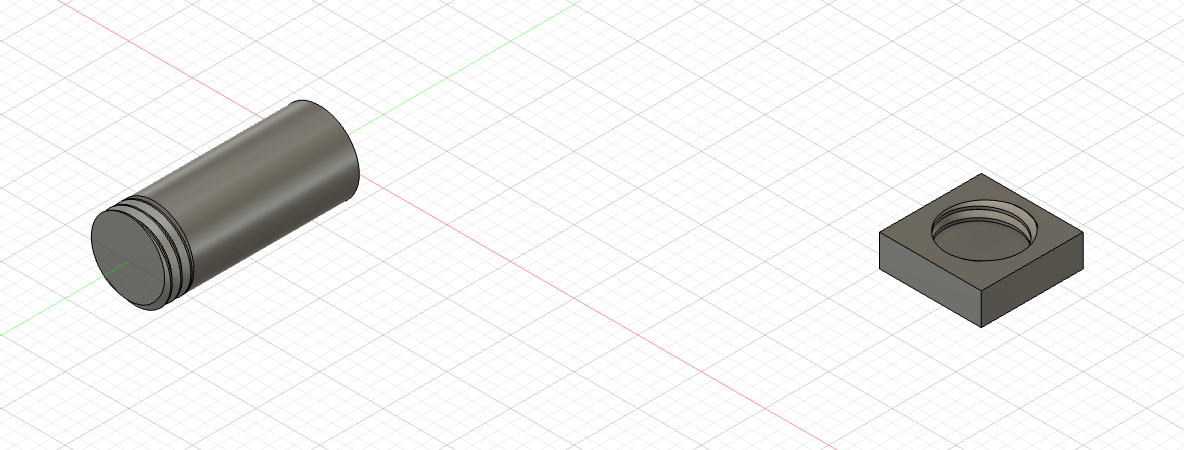
\includegraphics[width=0.8\textwidth]{LimitSwitchScrewTerminal.png}
        \caption{Test Prints for the Limit Switch Screw Terminal}
        \label{fig:LimitSwitchScrewTerminal}
    \end{figure}

    \subsection{Chassis Design \& Build}
    I have been in close talks with the ECE Machine Shop specifically Gregg and Jordan regarding the design and manufacturing of the robot. We been able to sort out many issues and design questions, the main questions being the following:

    \begin{itemize}
        \item Q: How to mount the omni-wheel onto the short motor axle?
        \item A: Custom axle to wheel hub should be built.
        \item Q: How to position the oxygen tank to lower the center of gravity to maintain robot stability and safety?
        \item A: We will be cutting a hole in the top level and lowering the oxygen tank to rest on the bottom level and be supported laterally by the top level (NOT shown in figure \ref{fig:RobotChassisBuild}).
        \item Q: Robot base material, what is best to ensure a low center of gravity?
        \item A: Medium-density fiberboard (MDF) is a great option and if needed we can add extra weight to the underside of the robot chassis.
        \item Q: How to support robot weight, is something extra like a caster wheel required under the center of the robot?
        \item A: MDF will be sturdy enought given our weight requirements.
    \end{itemize}

    The inital CAD design of the robot I designed can be seen in figure \ref{fig:Robot_CAD}. The current version of the robot chassis can be seen in figure \ref{fig:RobotChassisBuild}.

    \begin{figure}[ht!]
        \centering
        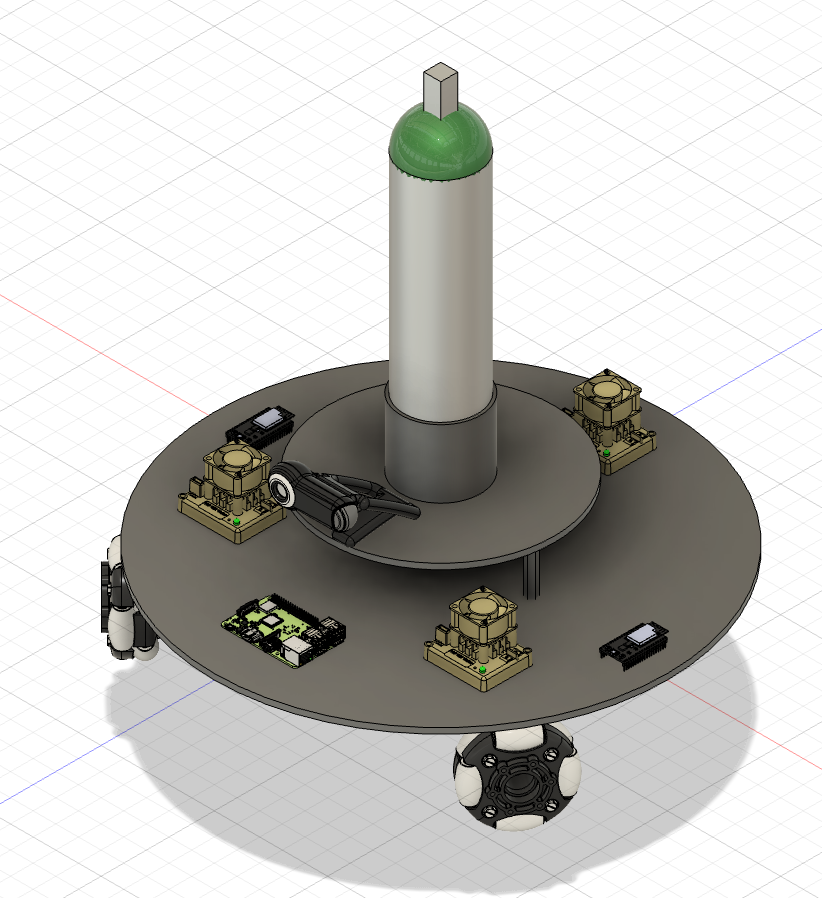
\includegraphics[width=0.8\textwidth]{Robot_CAD.png}
        \caption{Inital Robot CAD Assembly}
        \label{fig:Robot_CAD}
    \end{figure}

    \begin{figure}[ht!]
        \centering
        \includegraphics[angle=-90,width=0.8\textwidth]{RobotChassisBuild.png}
        \caption{Current Robot Chassis Assembly}
        \label{fig:RobotChassisBuild}
    \end{figure}

    \section{Testing/Verification}
    \label{sec:Testing}
    In terms of testing we will be using a modular testing plan, testing various subsystems individually. The week of March 25th is currently being used for testing of the accuracy for UWB triangulation. If testing passes then we can begin implementing the direction vector calculations that will help give the robot a direction to follow from the UWB data. Following that, testing of the power systems on the V1.1 of the PCB is also happening this week (our current bottleneck if the arrival of the PCBs), but we have all the components required, any issues will get revised and sent out in the fourth round of PCB orders. The hole in the top level of the chassis was completed on \today, and the robot motor and movement testing will occur during the week of April 1st. These are the main systems that require testing. Unfortunately, no further data has been gathered to show results in the form of graphs or tables but will be created within the next two weeks.

    \subsection{Contingency plans for failed tests}
    If testing fails on the UWB subsystem and we are unable to get the system to accurately triangulation location, we will be able to use the UWB for ranging which is already functional. With this and an angular vector provided from the Computer Vision subsystem we will still be able to accurately track a child.

    If testing fails on the power subsystem of the PCB, we have a Power Distribution Panel from an old FRC robot that can easily be used to help supply the power to the motors and we will breadboard our 5V supply power.

    \chapter{Conclusion}

    \section{Self-assessment}
    I do believe I have a slightly heavy workload for this project, but it is something I am aware of and okay with given the number of tasks required to complete this project. Following that, I believe we are slightly behind schedule. There are many unknowns we need to account for and need to give ourselves as much time as possible to sort them out.

    \section{Plans for remaining work}
    Please refer to the section \ref{sec:Testing} for the the short term plan. After that point it will be subsystem integration, where we will performing sensor fusions of the UWB and computer vision subsystem, and integrating the rest of the subsystems onto the chassis. I believe we are on track to finish the project, but it will definitely require all hands on deck to get it done properly.

    \section{Ethics and Safety}
    \subsection{Ethical Considerations}
    As we continue through the development of our project, we are unwavering in our dedication to abide by the ethical and safety principles outlined by the Association for Computing Machinery (ACM) and the Institute of Electrical and Electronics Engineers (IEEE). As we embark on this project, we pledge our commitment to adhere to these standards, ensuring that our actions and choices uphold the highest level of professionalism and integrity.

    As outlined in Section I of the IEEE Code of Ethics, we pledge to “uphold the highest standards of integrity, responsible behavior, and ethical conduct in professional activities” \cite{IEEE_2020}. We will prioritize safety in our design and adhere to ethical design practices. Educating the parents and caregivers about the robot’s use and limitations will allow for informed decision-making. Following relevant laws and regulations regarding this technology will also be a high priority.

    In the same Code of Ethics, outlined in Section III, we pledge to “strive to ensure this code is upheld by colleagues and co-workers” \cite{IEEE_2020}. We will support each other in ethical conduct and foster a culture of ethical behavior. Open communication will be established and encouraged to raise concerns and provide guidance to team members.

    \subsection{Safety Considerations}
    This project aligns with the safety principles outlined in the ACM Code of Ethics and Professional Conduct. Safety remains our number one priority and as outlined in Section 1.2 \cite{ACM_2018}, we will avoid negative consequences, especially when those consequences are significant and unjust. We will take careful consideration of potential impacts and minimize harm. In the context of this project, we will ensure that the robot’s design and operation prioritizes safety, especially to the children this product aims to assist. We will work to analyze potential risk and consider the robot’s mobility and interaction with its environment.

    As well as promoting safety, privacy is also a very important guideline that will be followed, which is outlined in Section 1.6. As professionals, we must safeguard the personal information of our users, especially if it involves children. As it relates to this project, we will ensure that no data will be collected and stored in an external location. Data collection will be minimized to only what is necessary for the robot to operate.

    One aspect of our project where safety must be considered is regarding the use of lithium batteries. We acknowledge the potential risks associated with the misuse of lithium batteries. We are committed to following the safety guidelines associated with the batteries we plan on using. More specifically, maintaining the battery’s temperature within the recommended range. Also, we are dedicated to the responsible disposal of batteries to ensure sustainability.

    Since we are incorporating motors into our design, we will deploy essential control systems to mitigate potential hazards such as collisions with the environment. Safe operation will be ensured with the use of sensors, vision systems, and warning systems.

    \bibliographystyle{IEEEtran}
    \bibliography{ref}

\end{document} % This is the end of the document